\documentclass[nooutcomes]{ximera}
%% handout
%% space
%% newpage
%% numbers
%% nooutcomes


\newcommand{\RR}{\mathbb R}
\renewcommand{\d}{\,d}
\newcommand{\dd}[2][]{\frac{d #1}{d #2}}
\renewcommand{\l}{\ell}
\newcommand{\ddx}{\frac{d}{dx}}
\newcommand{\dfn}{\textbf}
\newcommand{\eval}[1]{\bigg[ #1 \bigg]}

\usepackage{multicol}

\renewenvironment{freeResponse}{
\ifhandout\setbox0\vbox\bgroup\else
\begin{trivlist}\item[\hskip \labelsep\bfseries Solution:\hspace{2ex}]
\fi}
{\ifhandout\egroup\else
\end{trivlist}
\fi} %% we can turn off input when making a master document

\usepackage{fullpage}


\title{2.1:  The Idea of Limits}  

\begin{document}
\begin{abstract}		\end{abstract}
\maketitle


%problem 1
 \begin{problem} \hfil

	\begin{enumerate}

		\item What does a secant line to the graph of a  linear function look like?  What does a tangent line to the graph of a linear function look like? 

 \begin{freeResponse}		 
	
	A graph of a linear function $L$ defined by $L(x) = mx + b$, is a line, where $m$ is the slope of the line and $b$ is the $y$-intercept.
      
        For instance, here is the graph of a particular linear function
        \begin{image}
          \includegraphics[scale = 0.3]{"Graph of linear function".png}
        \end{image}

        If we draw a secant line between two points of this graph we have
        \begin{image}
          \includegraphics[scale = 0.3]{"Graph of linear function with secant line".png}
        \end{image}
        So the secant line is identical to the line itself.

        If we draw a tangent line at one point on this graph we have
        \begin{image}
          \includegraphics[scale = 0.3]{"Graph of linear function with tangent line".png}
        \end{image}
        So the tangent line is identical to the line itself.
\end{freeResponse}


		\item  What might a secant line and tangent line of the function $f$, defined by $f(x) = x^2$, look like?

\begin{freeResponse} \hfil
	\begin{image}
           \includegraphics[scale = 0.8]{"Graph of quadratic function with negative slope secant line".png}
         \end{image}
         \begin{image}
           \includegraphics[scale = 0.8]{"Graph of quadratic function with zero slope secant line".png}
         \end{image}
         \begin{image}
           \includegraphics[scale = 0.8]{"Graph of quadratic function with positive slope secant line".png}
         \end{image}
          \begin{image}
            \includegraphics[scale = 0.8]{"Graph of quadratic function with negative slope tangent line".png}
          \end{image}
          \begin{image}
            \includegraphics[scale = 0.8]{"Graph of quadratic function with zero slope tangent line".png}
          \end{image}
          \begin{image}
            \includegraphics[scale = 0.8]{"Graph of quadratic function with positive slope tangent line".png}
          \end{image}
          There is an important difference between secant lines and tangent lines!
          When we zoom in enough, \emph{at an appropriate point}, the tangent line looks \emph{nearly} indistinguishable from the graph itself:
          \begin{image}
            \includegraphics[scale = 0.3]{"Graph of zoomed in quadratic function".png}
          \end{image}
          Secant lines usually don't have this property.
	\end{freeResponse}

		\item In the graph below, is the given line a secant line or a tangent line at the point $A(a,f(a))$?
		\begin{image}
		 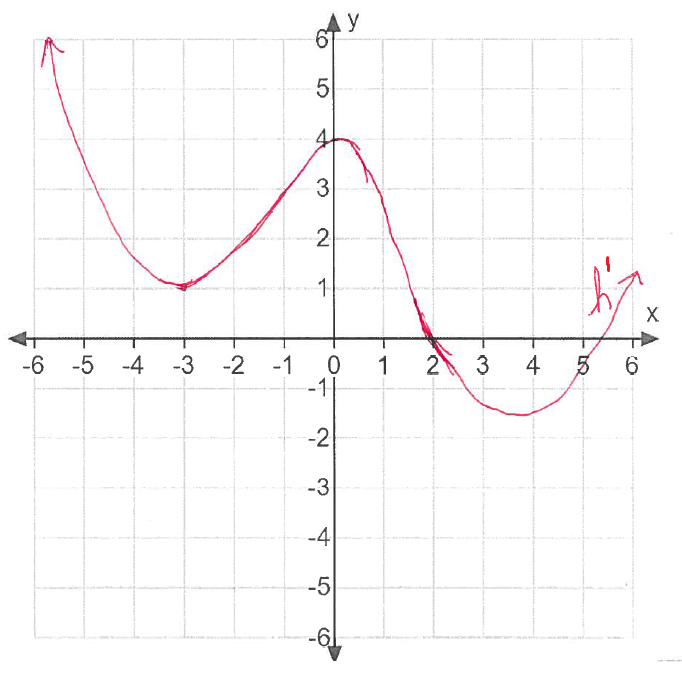
\includegraphics[scale = 0.7]{figure1.png}
		\end{image}

	\begin{freeResponse}
	This is a trick question!

        The given line is a tangent line at  $A(a,f(a))$---when we zoom in enough the graph is nearly indistinguishable from its tangent line at that point.
        But, it can also be considered a secant line through A and B.

        By convention however, since we have drawn the graph by emphasizing only one point of intersection we usually interpert such a line as a tangent line.
	      \end{freeResponse}
	\end{enumerate}

\end{problem}

%problem2
\begin{problem}
 Part of the given parabola can be used to model to ``position-time''graph of a ball thrown straight up into the air.  The graph gives the height of the ball in feet $t$ seconds after being thrown into the air.
  Use this graph, and the given function, to answer the following questions.
  \begin{image}
    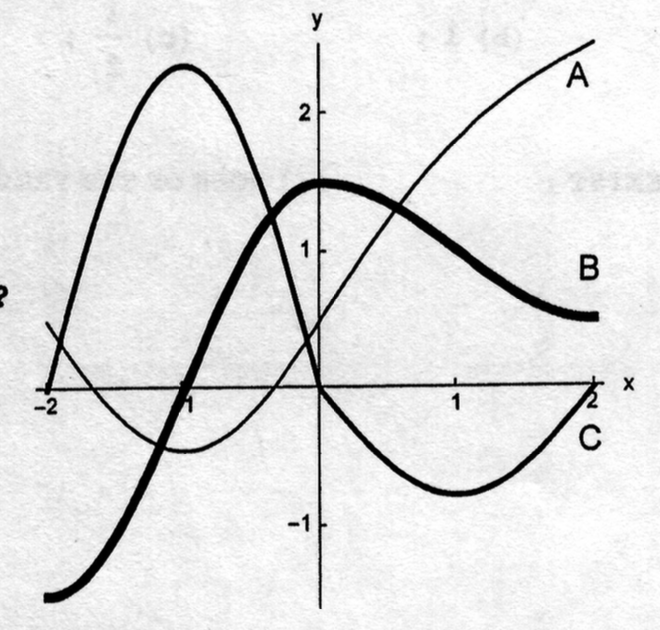
\includegraphics[scale = 0.8]{figure2.png}
  \end{image}
	
	
		\begin{enumerate}
		\item Mark the part of the parabola that can be used to model the position of the ball.		
		\begin{freeResponse} \hfil
       		 \begin{center}
       	  	 \includegraphics[scale = 0.4]{"Position time graph of ball".png}
        		\end{center}
		\end{freeResponse}		

		 \item  What are the units on the $t$ axis?  What are the units on the $y$ axis?
		 \begin{freeResponse}		 
	The units on the $t$ axis are ``seconds'' (for time), while the units on the $y$ axis are ``feet'' (for height).        
		\end{freeResponse}
			
		\item  If you were watching a movie of the ball being thrown, is the graph a picture of the path that the ball follows?  Why or why not?
		\begin{freeResponse}		 
	 No, the position-time graph is \emph{not} the path the ball follows.
        The graph shows the height of the ball at a given \emph{time}.
        The ball is thrown straight up and has no horizontal movement.
		\end{freeResponse}
	
		\item Let $f(t)$ done the height of the ball at time $t, t\geq 0$.  What is the height of the ball at time $t=0$?
		\begin{freeResponse}
		The height can be found by finding $f(0)$
		\begin{align*}
			f(0)&=-16(0)^2+128(0)+144 \\
			f(0)&=144\  \text{feet}
 			\end{align*}

		\end{freeResponse}
		
		\item  When will the ball hit the ground?
		\begin{freeResponse}		 
		The ball will hit the ground when the height $f(t)$ equals zero.
			\begin{align*}
			0&=-16t^2+128t+144 \\
			0&=-16(t^2-8t-9) \\
 			0&=-16(t+1)(t-9) \\
 			t&=-1,9 
 			\end{align*}
		The ball will hit the ground at $t=9$ or 9 seconds after the ball is thrown into the air.  
		\end{freeResponse}

		\item  What is the domain of the position function, $f$, of the ball?

		 \begin{freeResponse}
     	   The domain of $f$ is the interval $[0, 9]$.  The ball is released at $t=0$ and hits the ground at $t=9$.
     	   With this domain the position-time graph of the ball is given by
       		 \begin{center}
       	  	 \includegraphics[scale = 0.4]{"Position time graph of ball".png}
        		\end{center}
     	 \end{freeResponse}

		
		
		\item Use the table of values to find the average velocity of the ball between $t=8.9$ and $t=9$ seconds.
	\[
\begin{array}{|l|l|}
			\hline
			t & \approx f(t)  \\
			\hline
			8.9 & 15.84  \\
			\hline
			8.99 & 1.6  \\
			\hline
			8.999 & 0.159984  \\
			\hline
			8.9999 &  0.015998  \\
			\hline
			9 &  0  \\
			\hline
			\end{array}
		\]
  \begin{freeResponse}
    The average velocity of the ball between $t = 8.9$ seconds and $t = 9$ seconds is
    \[
       \frac{f(9) - f(8.9)}{9- 8.9} = \frac{0- 15.84}{0.1} = -158.4\  \text{feet per second}
    \]
  \end{freeResponse}


		\item  Use the table of average velocities to approximate the instantaneous velocity of the ball when it hits the ground.
			 \[
			\renewcommand*{\arraystretch}{2.5}	
			\begin{array}{|l|l|}
			\hline
			\text{Time Interval} & \text{Average Velocity}  \\
			\hline
			[8.9, 9] & \frac{f(9)-f(8.9)}{.1}=\frac{0-15.84}{.1}=-158.4  \\
			\hline
			[8.99,9] & \frac{f(9)-f(8.99)}{.01}=\frac{0-1.5984}{.01}=-159.84 \\
			\hline
			[8.999, 9] & \frac{f(9)-f(8.999)}{.001}=\frac{0-.159984}{.001}=-159.984 \\
			\hline
			[8.9999, 9] &  \frac{f(9)-f(8.999)}{.0001}=\frac{0-.0159998}{.0001}=-159.998  \\
			\hline
			\end{array} 
			\]
		

		\begin{freeResponse}
		 The instantaneous velocity of the ball hitting the ground appears to be $-160$ ft/sec.
		\end{freeResponse}
		
		
			
		\item    Use the  graph to determine if, at any moment in time, the ball has instantaneous velocity equal to 0.  Why or why not?

		\begin{freeResponse}		 
		 The ball has zero instantaneous velocity when the graph $f=f(t)$  has a tangent line with zero slope:
        \begin{image}
          \includegraphics[scale = 0.5]{"Position time graph with zero velocity".png}
        \end{image}
		\end{freeResponse}
		
		
		
		\item  For which times is the instantaneous velocity of the ball negative?
      What happens to the height of the ball when its velocity is negative?
      \begin{freeResponse}
        The instantaneous velocity of the ball is negative for $t > 4$:
        \begin{image}
          \includegraphics[scale = 0.5]{"Position time graph with negative velocity".png}
        \end{image}
        The height of the ball is decreasing at those times.
      \end{freeResponse}
			
		\end{enumerate}
			
\end{problem}
	
								
				
\end{document} 


















